\section{Einzelne Entscheidungsbäume}
\label{sec:construction}
\begin{figure}
    \centering
    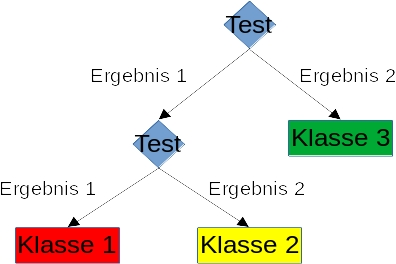
\includegraphics[width=0.5\linewidth]{images/entscheidungsbaum.jpg}
    \caption{Beispiel eines binären Entscheidungsbaums mit 3 möglichen Ergebnissen.}
    \label{fig:entscheidungsbaum}
\end{figure}
Der einzelne Entscheidungsbaum ist eine rekursive Datenstruktur, um Entscheidungsregeln darzustellen. Jedem inneren Knoten ist ein \textit{Test} zugeordnet, der eine arbiträre Anzahl von sich gegenseitig
ausschließenden Ergebnissen hat. Das Ergebnis bestimmt mit welchem Kindknoten fortgefahren wird \cite{quinlan1990decision}. Abbildung \ref{fig:entscheidungsbaum} zeigt einen Entscheidungsbaum, in dem jeder Test
zwei mögliche Ergebnisse hat, einen binäreren Entscheidungsbaum.
\newline
\newline
Beim maschinellen Lernen werden Entscheidungsbäume aus Trainingsmengen generiert. Die Trainingsmenge besteht aus Feature-Mengen, die mit Klassen beschriftet sind \cite{steinbergCART}. Sie sollte möglichst repräsentativ
für die Gesamtmenge des Trainierten sein, d. h. im Falle der Handgesten, sollten möglichst alle Handgesten, Lichtverhältnisse und Geschwindigkeiten abgedeckt sein. Daneben müssen die Features eine eindeutige
Partitionierung aller Klassen ermöglichen. Außerdem sollte die Feature-Menge keine irrelevanten Features enthalten, da diese die Effektivität stark beeinträchtigen können. Sind alle Anforderungen erfüllt, ist eine
gute Generalisierung möglich \cite{pei1998feature}.
\newline
\newline
Es gibt verschiedene Algorithmen, um Entscheidungsbäume zu erzeugen, z. B. \texttt{ID3} \cite{quinlan1986induction}, \texttt{C4.5} \cite{quinlan2014c4}
oder \texttt{CART} \cite{breiman1984classification}. Das Grundprinzip ist dabei immer das gleiche. Partitioniere die Trainingsmenge, sodass möglichst nur Einträge mit der
gleichen Beschriftung in einer Partitionierung enthalten sind. Die Algorithmen unterscheiden sich in ihrer Strategie. Der naive Ansatz ist alle möglichen Entscheidungsbäume zu generieren und davon den besten auszuwählen.
Das ist aber bei großen Feature- und Trainingsmengen sehr rechenaufwändig. Aus diesem Grund werden Heuristiken verwendet, die schnell sind aber nicht optimal sein müssen \cite{quinlan1986induction}.
\newline
\newline
Scikit-Learn implementiert eine optimierte Version des \texttt{CART} (Classification and Regression Trees) Algorithmus \cite{ScikitLearnCART}.
CART partitioniert die Trainingsmenge und wählt dabei immer lokal die beste Teilung aus, d. h. es wird der beste Schwellenwert ausgewählt, der die Menge teilt.
\begin{lstlisting}[label=lst:CARTtreeGrowing,caption={Skizze vereinfachten Baumwachstumsalgorithmuses \cite{steinbergCART}.}]
BEGIN:
Assign all training data to the root node
Define the root node as a terminal node

SPLIT:
New_splits=0
FOR every terminal node in the tree:
    If the terminal node sample size is too small or all instances in the node belong to the same target class goto GETNEXT
    Find the attribute that best separates the node into two child nodes using an allowable splitting rule
    New_splits+1

GETNEXT:
NEXT
\end{lstlisting}
Listing \ref{lst:CARTtreeGrowing} skizziert den vereinfachten Baumwachstumsalgorithmus von CART. Der Algorithmus teilt solange die Trainingsmenge, bis keine weitere Teilung mehr möglich ist oder in allen Knoten nur
Einträge mit der gleichen Beschriftung enthalten sind. Danach werden sukzessiv Teilbäume entfernt, die nach einer Bewertungsfunktion, z. B. Zuwachs der Klassifizierungsgenauigkeit, unterhalb eines vordefinierten
Schwellenwert liegen \cite{steinbergCART}.